\documentclass{../template/labo}
\usepackage[utf8x]{inputenc}

\usepackage[frenchb]{babel}
\usepackage[T1]{fontenc}

\usepackage{graphicx}
\usepackage{amssymb}
\usepackage{amsmath}
\usepackage{wasysym} %smiley
\usepackage{hyperref}% hyperliens
\usepackage{tikz}
\usetikzlibrary{babel,positioning,calc}
\usepackage[]{circuitikz}
\usepackage{textcomp}
% \usepackage{minted}
\usepackage[long]{datetime}
\usepackage{gensymb} % \ohm, celsius
\usepackage{framed}
\usepackage{pdfpages}
\usepackage{todo}
\usepackage{paralist}
\usepackage{multicol}

\usepackage{mathastext} % math as standfard text : units are respecting typography conventions.
\usepackage{fancyhdr} %en-tête
\usepackage{qrcode}
\usepackage{pgfplots} %for latex grid

\langexam{frenchb}

\correction{false}
%\correction{true}

\author{The Fantastic Four} %<3


%% fancy header & foot
\pagestyle{fancy}
\lhead{[ELEC-H-301] Électronique appliquée\\ LABO \no 6 : Instrumentation d'un moteur\ifthenelse{\boolean{corrige}}{~-- corrigé}{}}
\rhead{v1.0.4\\ page \thepage}
\cfoot{}
%%

\pdfinfo{
/Author (ULB -- BEAMS)
/Title (LABO 1 ELEC-H-301, Filtrage)
/ModDate (D:\pdfdate)
}

\hypersetup{
pdftitle={LABO 6 [ELEC-H-301] Électronique appliquée: Instrumentation d'un moteur},
pdfauthor={ULB - BEAMS},
pdfsubject={Instrumentation d'un moteur}
}

%\date{\vspace{-1cm}\mydate\today}
%\title{\vspace{-2cm} Labo \no 6\\ Électronique appliquée [ELEC-H-301]\\Réalisation d'un ampli à transistor\ifthenelse{\boolean{corrige}}{~\\Corrigé}{}}

%\author{\vspace{-1cm}}%\textsc{Yannick Allard}}

\setlength{\parskip}{0.5cm plus4mm minus3mm} %espacement entre §
\setlength{\parindent}{0pt}


\begin{document}

\tptitle{}{Séance 6~: Instrumentation d'un moteur}

\section{But de la manipulation}

L'objectif principal de cette manipulation est de réaliser une mesure de courant sur un moteur
électrique en rotation entrainant une hélice.\\
Pour ce faire, vous serez amenés à utiliser un amplificateur différentiel afin d'éliminer les parasites
dus à l'alimentation.\\
Après avoir filtré le courant, vous devrez réaliser un système de protection afin de limiter le courant
absorbé par le moteur, en stoppant ce dernier si une valeur limite venait à être dépassée

\section{Pré-requis}
Ce labo fait intervenir des notions de filtrage et d'amplifications, il est donc nécessaire de relire les
labos 1 et 2 ainsi que les TPs 1 à 3.\\
De plus, les sections du cours sur l'amplification différentielle sont supposées connues. Ce labo fait
également appel aux notions sur les portes logiques de base vues au labo 5.

\section{Matériel}
En plus du matériel classique de laboratoire (multimètre, oscilloscope, générateur de fonction, câbles, etc.), cette séance nécessite les composants suivants:
\begin{itemize}
\item un AOP TLE2061 et les résistances pour le montage du 7.3
\item un comparateur MCP6541, un bistable RS HEF4043
\item l'hélice avec l'ampli de puissance integré
\item un condensateur dimensionné à la question 17.
\end{itemize}

\newpage
\section{Préliminaire théorique} %{\normalsize{(1 point)}}}
Il vous est recommandé de répondre aux exercices des points 1.3, 2.3 et 3 avant d'arriver au
laboratoire.

\section{Objectifs}
A la fin de ce laboratoire, vous devez être capable :

\begin{itemize}
\item de justifier l'utilité d'une amplification différentielle
\item de dimensionner et réaliser un amplificateur différentiel à quatre résistances
\item d'établir la table de vérité de circuits logiques simples
\item de dimensionner un filtre afin de ne conserver que le signal utile.
\end{itemize}

\section{Introduction au contrôle de moteur}
\subsection{Introduction}

Tout au long de ce laboratoire, nous allons étudier un système permettant de faire tourner une hélice à
vitesse variable :

\begin{center}
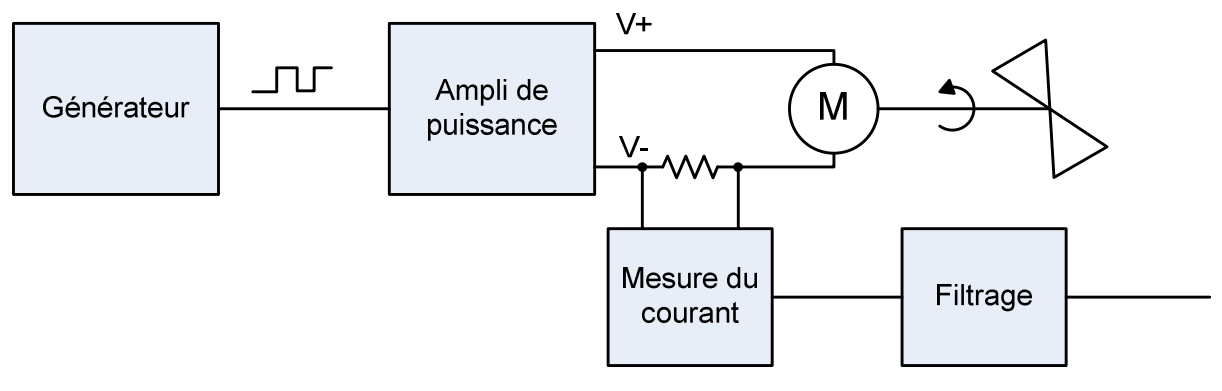
\includegraphics[width=12cm]{sch1}
\end{center}

Un générateur, configuré de sorte à fournir une onde en créneaux, alimente un moteur à courant
continu à travers un ampli de puissance. En jouant sur le signal du générateur, il est
possible de modifier la vitesse de rotation du moteur.
Une hélice est connectée au moteur et génère un couple résistant freinant ce dernier.
Afin de s'assurer que le moteur ne sorte pas de ses limites de fonctionnement, vous devez
mesurer le courant circulant dans le circuit ; ceci se fera à l'aide d'une mesure de la
tension aux bornes d'une résistance connue de $0.1\Omega$. Cette mesure sera ensuite filtrée
afin de supprimer les effets à haute fréquence.

\subsection{Onde carrée : définitions}
La commande de l'amplificateur de puissance se fait à l'aide d'une onde carrée. Diverses
définitions sont associées à ce type de signal :

\begin{center}
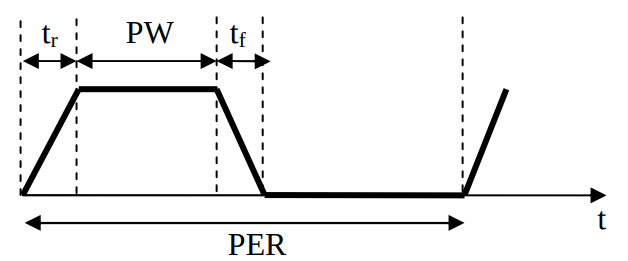
\includegraphics[width=10cm]{sch2}
\end{center}

Les différents temps caractéristiques sont les suivants :

\begin{itemize}
\item $PW$ (Pulse Width) est la durée de l'état haut
\item $PER$ est la période du signal
\item $t_r$ (rising time) est le temps de montée
\item $t_f$ (falling time) est le temps de descente
\end{itemize}

Dans la majorité des cas, y compris ici, les temps de montée et de descente sont négligeables.
Une autre caractéristique du signal est son rapport cyclique :\\

il est défini comme $D = \frac{PW}{PER}$ et correspond à la proportion du temps passée à l'état haut.

\subsection{Modélisation du moteur}

Un moteur à courant continu peut en première approximation être vu comme une inductance. Dans
le cas présent, celle-ci est de $7mH$. Le bobinage fait également apparaître une résistance de
$7\Omega$.
En négligeant la résistance de mesure de $0.1\Omega$, nous arrivons au circuit RL suivant :

\begin{center}
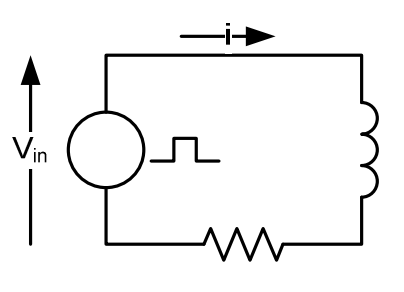
\includegraphics[width=7cm]{sch3}
\end{center}
\vspace*{2cm}

\subsection{Prédéterminations}
\Question{Tracez l'évolution temporelle du courant si celui-ci est initialement nul et que la tension $V_{in}$
varie brutalement de $0V$ à $5V$ à l'instant initial.}{}
\Question{Supposons maintenant que l'entrée est une onde carrée de rapport cyclique 50\%, tracez
l'évolution du courant pour une fréquence de commutation de $10Hz$ et de $10kHz$. Quel est
l'effet de la fréquence ?}{}
\Question{En gardant une fréquence de modulation de $10kHz$, calculez la valeur moyenne du courant
en régime établi pour un rapport cyclique de 20\%, 50\%, 80\%. Pour ce faire, calculez d'abord
la valeur moyenne de la tension. Pourquoi les autres composantes de $V_{in}$ ne vont-elles pas
influencer la valeur moyenne du courant ?}{}

\section{Mesure du courant}
\subsection{Introduction}
La différence de potentiel autour de la résistance de mesure donne une image du courant circulant dans
le moteur. En mesurant cette différence de potentiel, vous serez à même de connaître le courant. Afin
d'obtenir une mesure claire, vous devrez amplifier le signal à l'aide d'un montage adéquat.

\subsection{Mesure du courant à une voie}

\Question
{Alimentez l'ampli de puissance avec le $+5V/0V$ du protoboard, et fournissez à son entrée $IN2$
une onde en créneaux d'une amplitude de $5V$ et d'une fréquence de $1kHz$. Le schéma de la
carte est donné en annexe. N'oubliez pas de connecter les bornes GND à la masse.
}{}

\Question{
Vérifiez l'effet du rapport cyclique et de la fréquence de modulation sur la vitesse de rotation
de l'hélice. Quel paramètre est le plus déterminant ?
}{}

\Question{
Visualisez le courant en connectant l'oscilloscope à une des deux bornes de la résistance
(bornes ISENSE de la carte). Que constatez-vous ? Justifiez vos résultats.
}{}

\Question{
En utilisant deux sondes, mesurez la différence de potentiel sur la résistance.
Vos résultats sont-ils meilleurs ?
}{}

\Question{
Justifier pourquoi une amplification classique (montage non-inverseur) ne peut dès lors pas
fonctionner correctement.
}{}

\subsection{Mesure différentielle}

Les résultats peuvent être fortement améliorés en utilisant une mesure différentielle.
Le schéma de principe de ce type d'amplification est le suivant :

\begin{center}
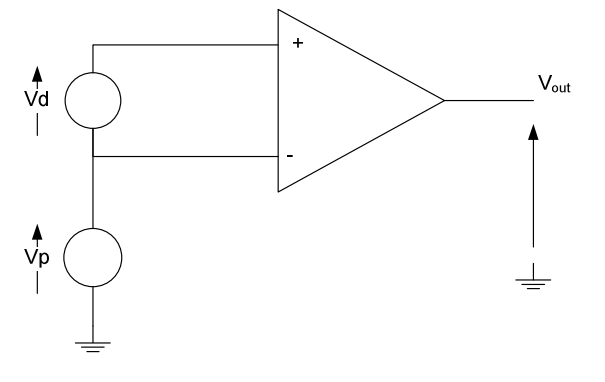
\includegraphics[width=10cm]{sch4}
\end{center}

Le principe est alors d'amplifier la différence de potentiel Vd autour de la résistance et de supprimer
au mieux la tension Vp. Cette tension représente éventuellement des parasites, mais également divers
couplages et est induite par le fait qu'aucune des bornes d'entrée n'est à la masse.

En pratique, nous utiliserons plutôt la notion de tension de mode commun :

$$V_{MC}=\frac{V_+ + V_-}{2} = V_p + \frac{V_d}{2}$$

Le schéma devient alors le suivant :

\begin{center}
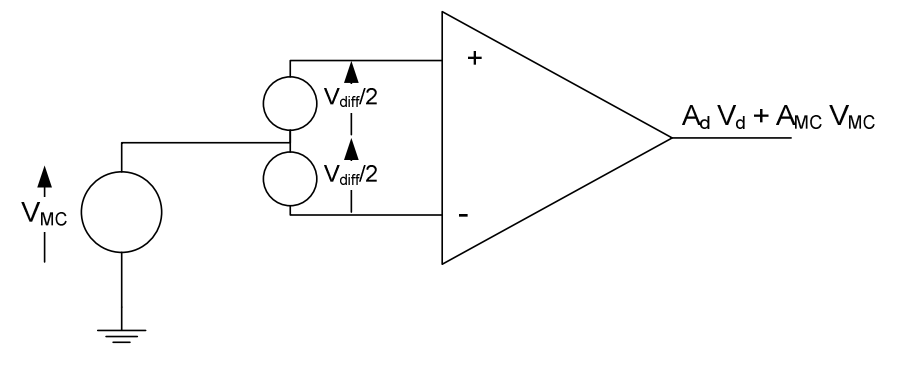
\includegraphics[width=10cm]{sch5}
\end{center}

L'amplificateur différentiel est chargé de multiplier la différence de potentiel $V_d$ par un facteur $A_d$ tout
en supprimant au mieux la tension de mode commun $V_{MC}$, qui dans notre cas correspond à la tension
variable à la sortie de l'ampli de puissance.
Malheureusement, une fraction de cette tension se retrouve tout de même à la sortie, ce qui se marque
par le gain $A_{MC}$.

Le montage différentiel le plus simple s'articule autour d'un ampli-op et de quatre résistances :

\begin{center}
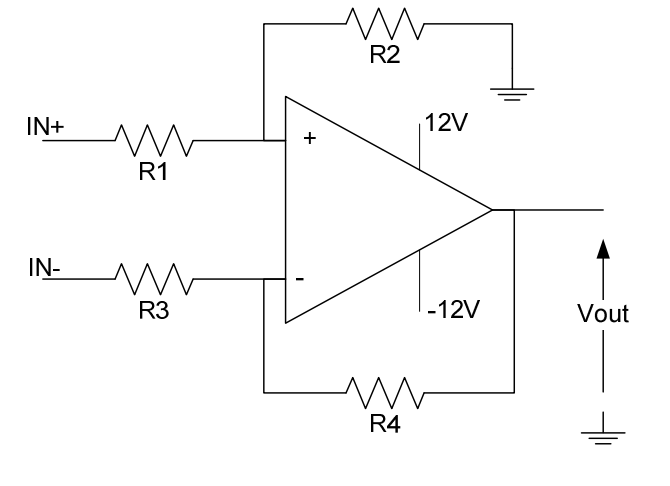
\includegraphics[width=10cm]{sch6}
\end{center}

\subsection{Prédéterminations}
\Question{
Exprimez Vout en fonction de Vd et VMC.
}{}

\Question{
En supposant que $R_1 = R_3$, donner une condition sur $R_2$ et $R_4$ pour que la tension de mode commun soit complètement rejetée de la mesure.
}
{}

\Question{
Sachant que le moteur absorbe 500mA au maximum, que $R_1 = 1k\Omega$ et que l'on désire une
sortie d'une amplitude de 5V, dimensionnez le montage.}
{}

\Question{
En quoi vos résultats sont-ils dégradés si la valeur de R4 présente une erreur de 5\% ?
}{}

\subsection{Manipulation}
\Question{
A l'aide d'un ampli TLE2061, réalisez le câblage du montage. Alimentez l'ampli en $+12V/-12V$. Les résistances $R_1$ et $R_3$ sont déjà sur la carte et valent $1k\Omega$
}
{}

\Question{
Observez la tension de sortie. Est-elle encore perturbée par la tension de mode commun ?
}{}

\section{Filtrage}
Lorsque nous réalisons une mesure de courant, il n'est pas rare que seule la valeur moyenne nous
intéresse. Afin de supprimer les effets dus à la commutation, nous allons filtrer passe-bas la mesure.
Pour la suite, fixez la fréquence de découpage à 5 kHz.
Le filtre RC, représenté ci-dessous, a déjà été étudié auparavant au labo 1. Il s'agit d'un filtre du
premier ordre :

\begin{center}
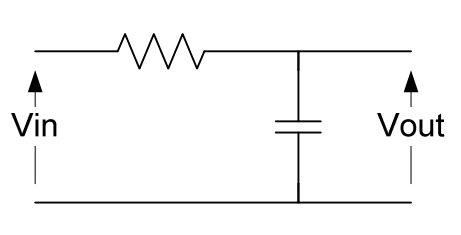
\includegraphics[width=8cm]{sch7}
\end{center}

\subsection{Prédéterminations}

\Question{
Établissez la fonction de transfert du circuit
}{}

\Question{
Déduisez-en le tracé asymptotique de ses courbes de Bode
}{}

\Question{
Une règle de bonne pratique stipule de choisir une fréquence de coupure égale au dixième de
la fréquence la plus basse à supprimer. Justifiez cette règle et dimensionnez le condensateur
sachant que la résistance est de $10k\Omega$.
}{}

\subsection{Manipulation}
\Question{
Observez la transformée de Fourier (FFT) du courant non filtré : à quoi correspondent les raies
les plus importantes ?
}{}

\Question{
Réalisez votre filtre RC et observez le courant filtré ainsi que sa FFT. Discutez quant à
l'efficacité de ce montage.
}{}

\section{Dispositif de protection}
\subsection{Détection de seuil}
Afin de protéger le montage contre les surcourants, nous allons réaliser un système de protection
basique. Son principe est d'observer le courant filtré et lorsque cette valeur dépasse un seuil défini, de
couper le circuit d'alimentation.

Commençons par détecter lorsque le courant dépasse une valeur limite. Ceci peut se faire à l'aide
d'un ampli-op monté en comparateur :

\begin{center}
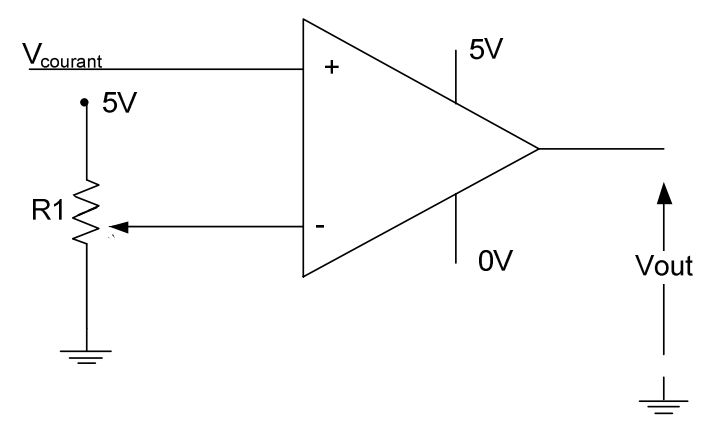
\includegraphics[width=10cm]{sch8}
\end{center}

Dès que la tension Vcourant sortant du filtre devient supérieure à la tension imposée à la borne négative
de l'ampli-op, la sortie bascule de 0V à 5V. Un potentiomètre permet de régler le seuil.

\subsection{Manipulation}

\Question{
Réalisez le module de détection à l'aide d'un comparateur MCP6541, spécialement prévu pour
être alimenté en +5V/0V.
}{}

\Question{
Réglez le montage de sorte à ce que la sortie bascule lorsque le courant atteint 80\% de sa
valeur maximale (obtenue en bloquant le moteur à la main lorsque ce dernier est alimenté par
le plus grand rapport cyclique possible).
}{}

\Question{
Testez votre montage en reliant la sortie de l'amplificateur à une des LED du protoboard.
}{}

\subsection{Coupure de l'alimentation}

La dernière étape est de réaliser un module coupant l'alimentation lorsque la sortie du comparateur
bascule et empêchant au moteur de redémarrer tant que l'utilisateur ne le réactive pas volontairement.
Pour ce faire, nous allons utiliser un circuit logique bien connu nommé le bistable RS, intégré dans le
circuit HEF4043.

\begin{center}
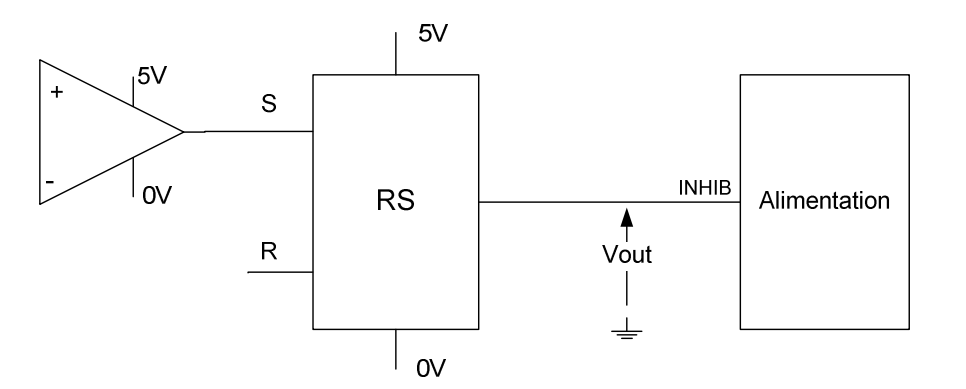
\includegraphics[width=11cm]{sch9}
\end{center}

Le principe de fonctionnement de ce circuit est noté dans la notice du circuit, le principe de base est
rappelé ici :

\begin{itemize}
    \item Lorsque que l'entrée S passe de l'état bas (0V) à l'état haut (5V), la sortie est fixée l'état haut.
    \item Lorsque que l'entrée R passe de l'état bas (0V) à l'état haut (5V), la sortie est fixée l'état bas.
    \item Lorsque les deux entrées sont à l'état haut, la sortie est fixée à l'état haut.
    \item Lorsque les deux entrées sont à l'état bas, la sortie conserve sa dernière valeur. Il s'agit de l'état de base du circuit.
\end{itemize}

La sortie du RS est connectée à l'entrée INHIB de la carte d'alimentation. Lorsque cette entrée est à
l'état haut, l'alimentation est coupée.

\subsection{Manipulation}

\Question{
A l'aide de la notice, justifiez la table de vérité du bistable RS.
}{}

\Question{
Réalisez le montage en utilisant n'importe lequel des 4 bistables présent dans le circuit
HEF4043 (veillez à mettre l'entrée OE à l'état haut).
}{}

\Question{
Reliez l'entrée R à un commutateur du protoboard, de sorte à pouvoir relancer le moteur après
qu'il s'est coupé.
}{}

\Question{
Testez votre montage : vérifiez que le moteur se coupe lorsque vous bloquez l'hélice et qu'il
redémarre après activation de l'interrupteur.
}{}


\section{Annexe}
Le générateur de fonction n'est pas suffisamment puissant que pour alimenter un moteur. Comme c'était le cas
pour l'amplificateur audio, nous allons utiliser un circuit d'amplification de puissance.
Cette fois, nous allons utiliser un amplificateur à commutation, ce qui signifie qu'il fournit à sa sortie une onde
carrée et non un signal continu.


Son schéma de principe est tracé ci-dessous.

\begin{center}
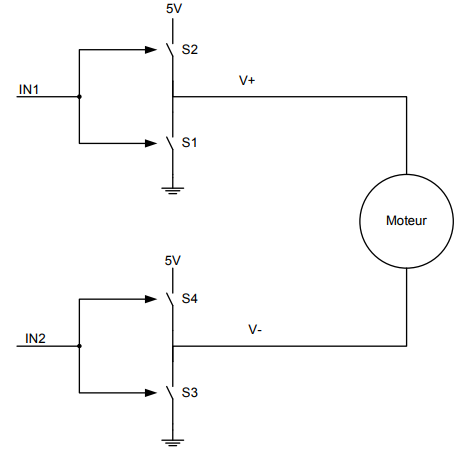
\includegraphics[width=9cm]{sch10}
\end{center}

Les signaux IN1 et IN2 sont des grandeurs binaires qui valent soit 0V (état bas, ou 0), soit 5V (état haut, ou 1). Il
s'agit de la commande de l'amplificateur.
Les interrupteurs S1 et S3 sont actifs (passants) lorsque IN1 ou IN2 sont à l'état haut, alors S2 et S4 sont actifs
lorsque IN1 ou IN2 sont à l'état bas.


Chacune des deux bornes de sortie V+ et V- est donc reliée soit à la masse, soit à la tension d'alimentation de
5V. Le moteur sera dès lors commandé en -5V/0V/5V. Par défaut les deux entrées sont à l'état bas.
L'avantage de ce système par rapport à une amplification classique est qu'il possède un rendement élevé. En
première approximation, aucune puissance n'est dissipée dans les interrupteurs, ce qui implique que le
rendement de l'alimentation est proche de 100\%.


Une entrée supplémentaire, nommée INHIB, permet de désactiver l'alimentation en forçant 0V sur les deux
pattes de sortie quel que soit l'état des entrées.


Le schéma d'implantation est donné ci dessous. Nous pouvons y voir les divers connecteurs de la carte. En plus
des diverses entrées de commande, nous y trouvons également les bornes d'alimentation à relier au 0V et au 5V
du protoboard ainsi que les connecteurs du moteur et de mesure.


Les bornes Vsense permettent de mesurer la tension aux bornes du moteur.


Les bornes Isense sont connectées à la résistance de $0.1\Omega$ de mesure du courant.

\begin{center}
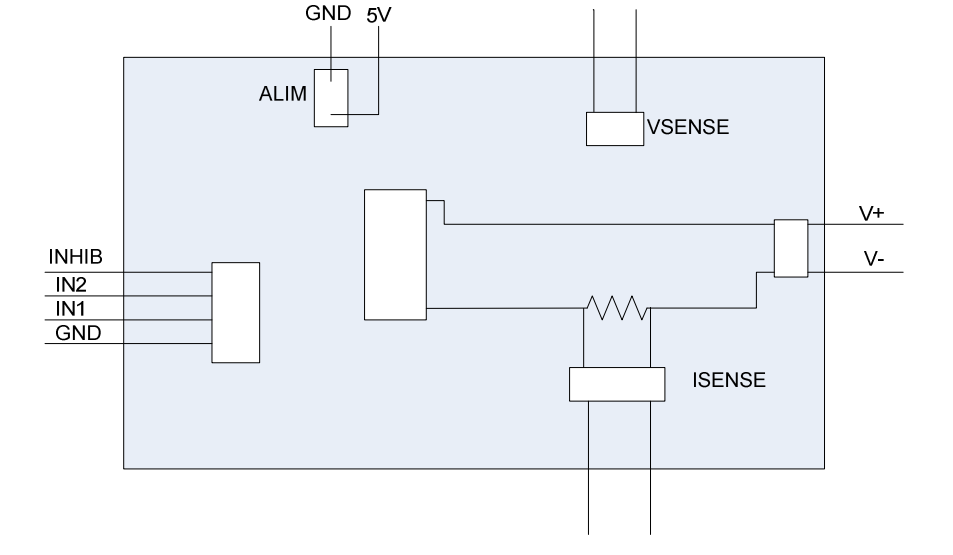
\includegraphics[width=15cm]{sch11}
\end{center}

\end{document}
